\xchapter{PRIEDAI}

\xsection{Priedas nr. 1: Klausimynas prieš testavimą}
\noindent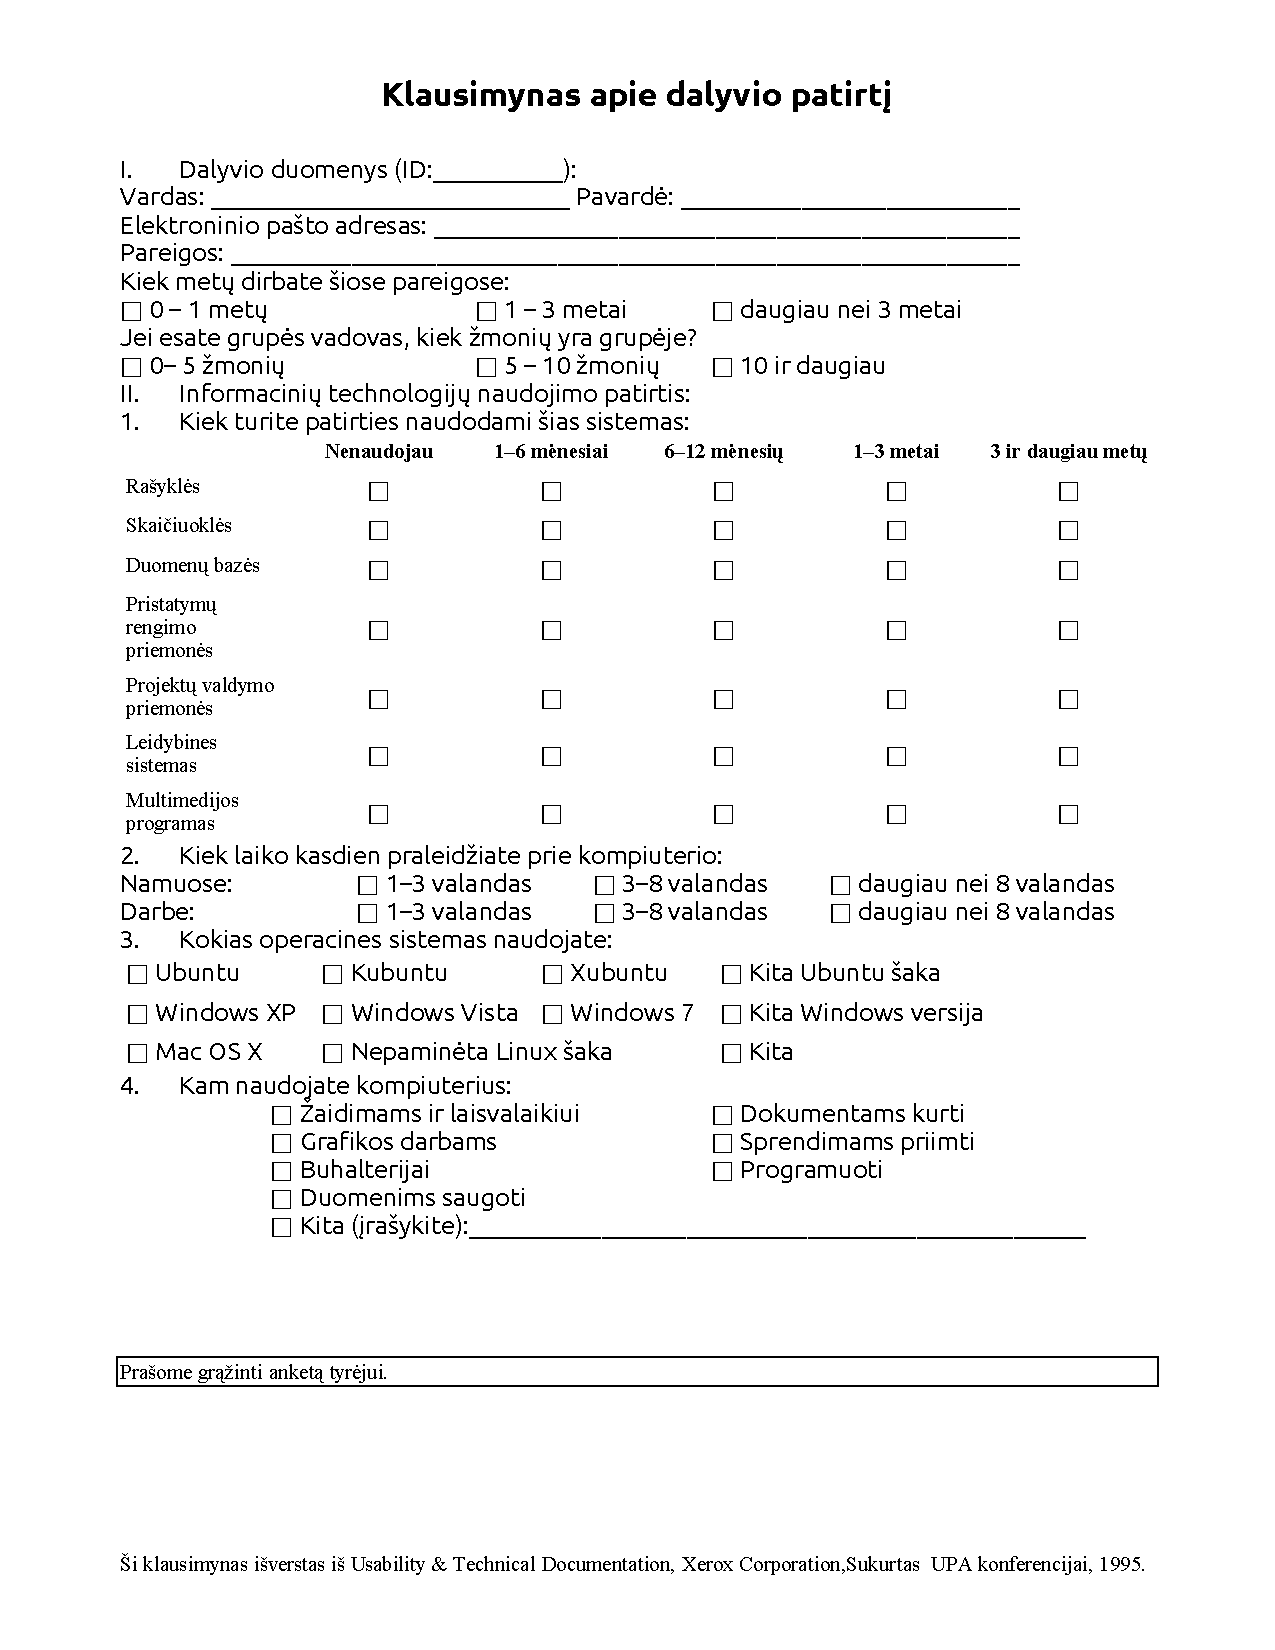
\includegraphics[scale=0.75]{./4/pdfs/klausimynas0.pdf}

\xsection{Priedas nr. 2: Klausimynas po testavimo}
\noindent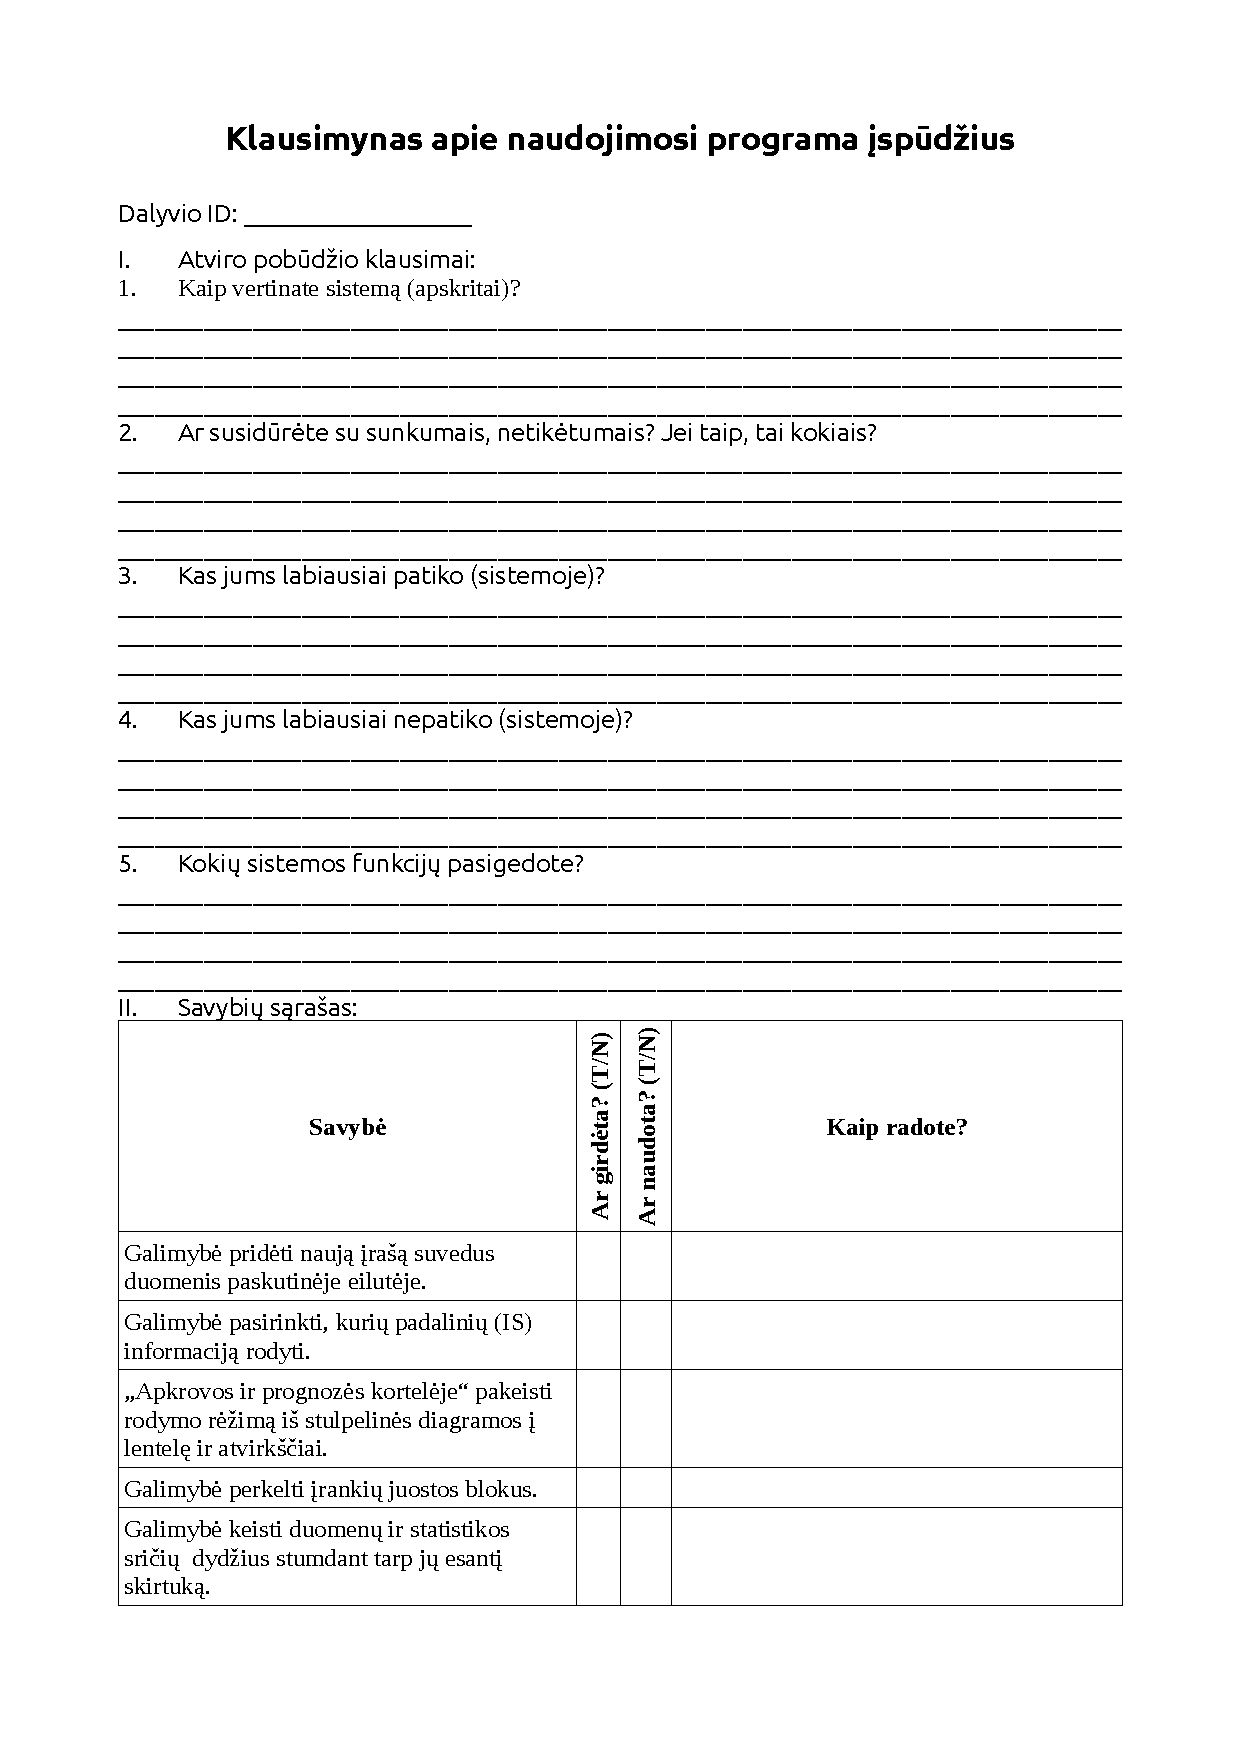
\includegraphics[scale=0.85, page=1]{./4/pdfs/klausimynas1.pdf}

\newpage
\noindent\includegraphics[scale=0.85, page=2]{./4/pdfs/klausimynas1.pdf}

\newpage
\noindent\includegraphics[scale=0.85, page=3]{./4/pdfs/klausimynas1.pdf}

\xsection{Priedas nr. 3: Sutikimo forma}
\hspace{-4.0cm}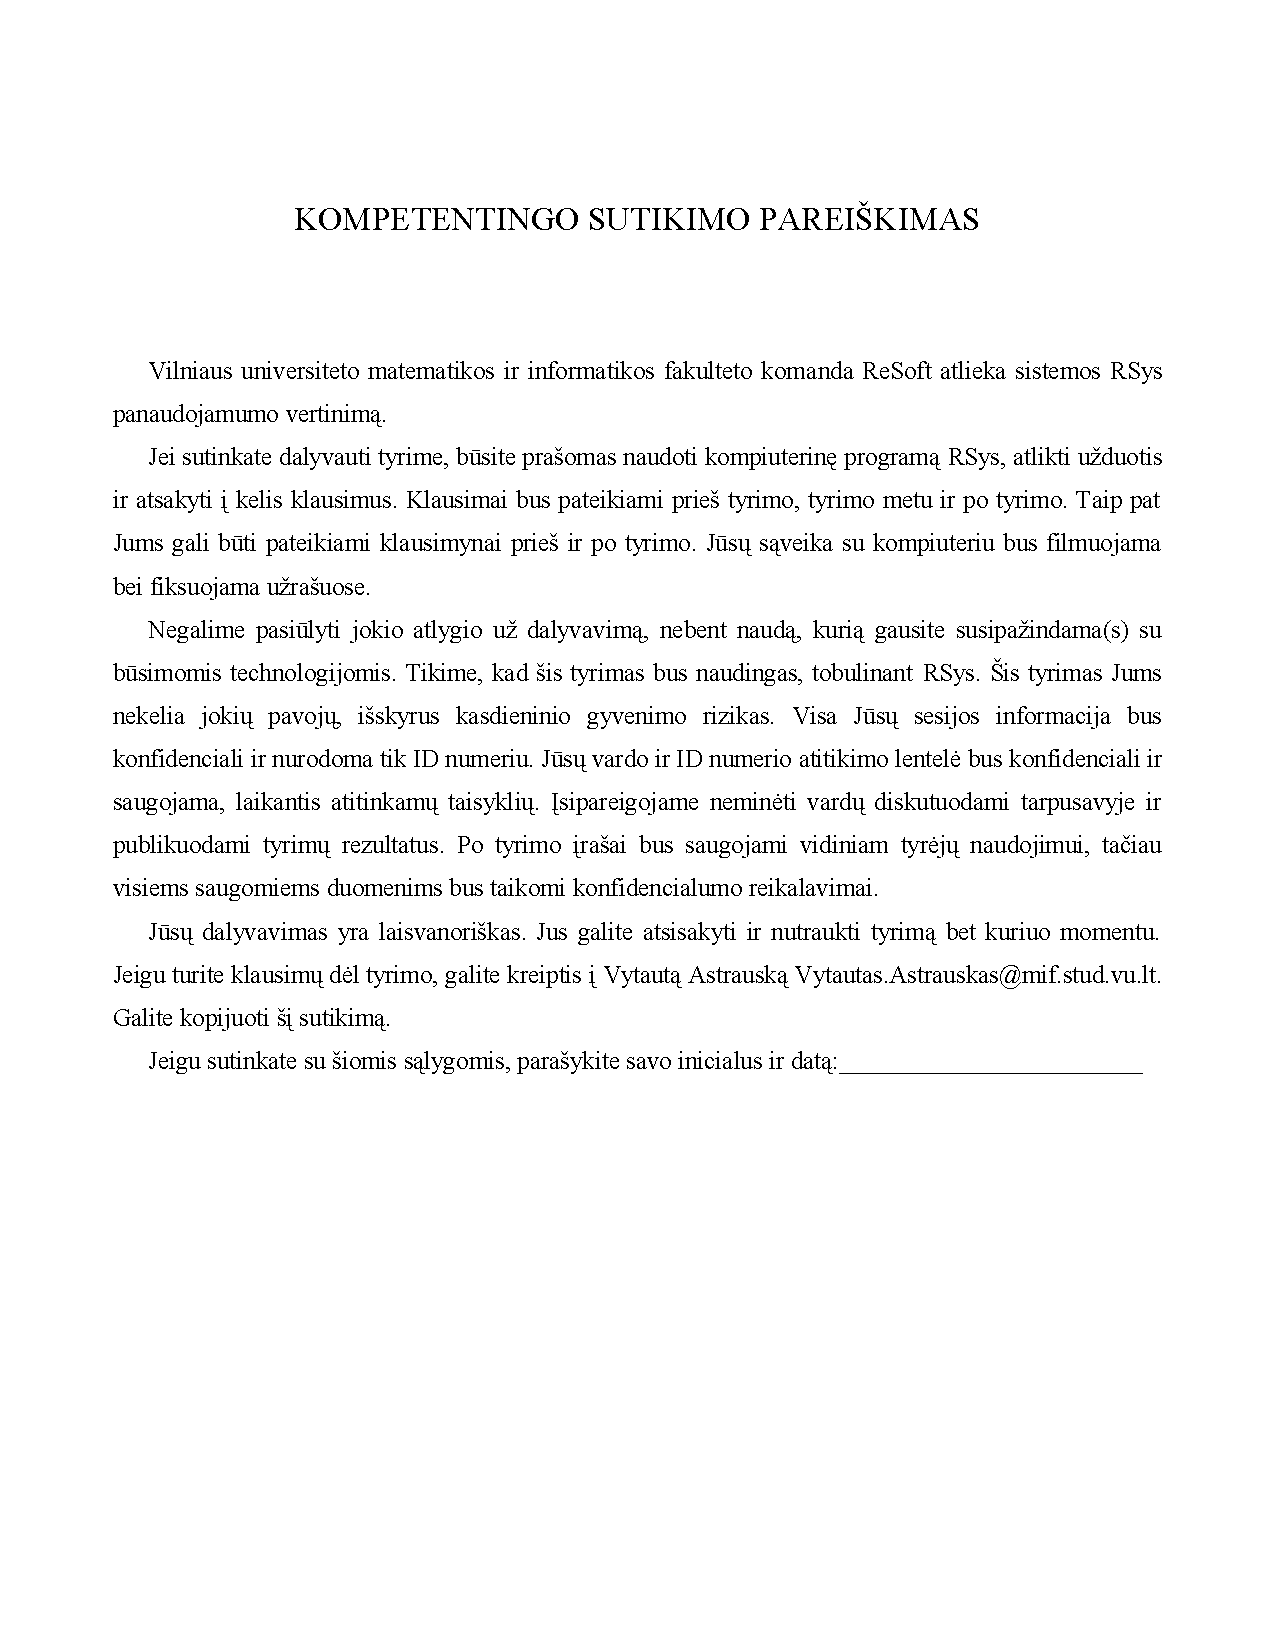
\includegraphics[scale=1.00]{./4/pdfs/sutikimas.pdf}

\xsection{Priedas nr. 4: Užduoties aprašymas}
\hspace{-4.0cm}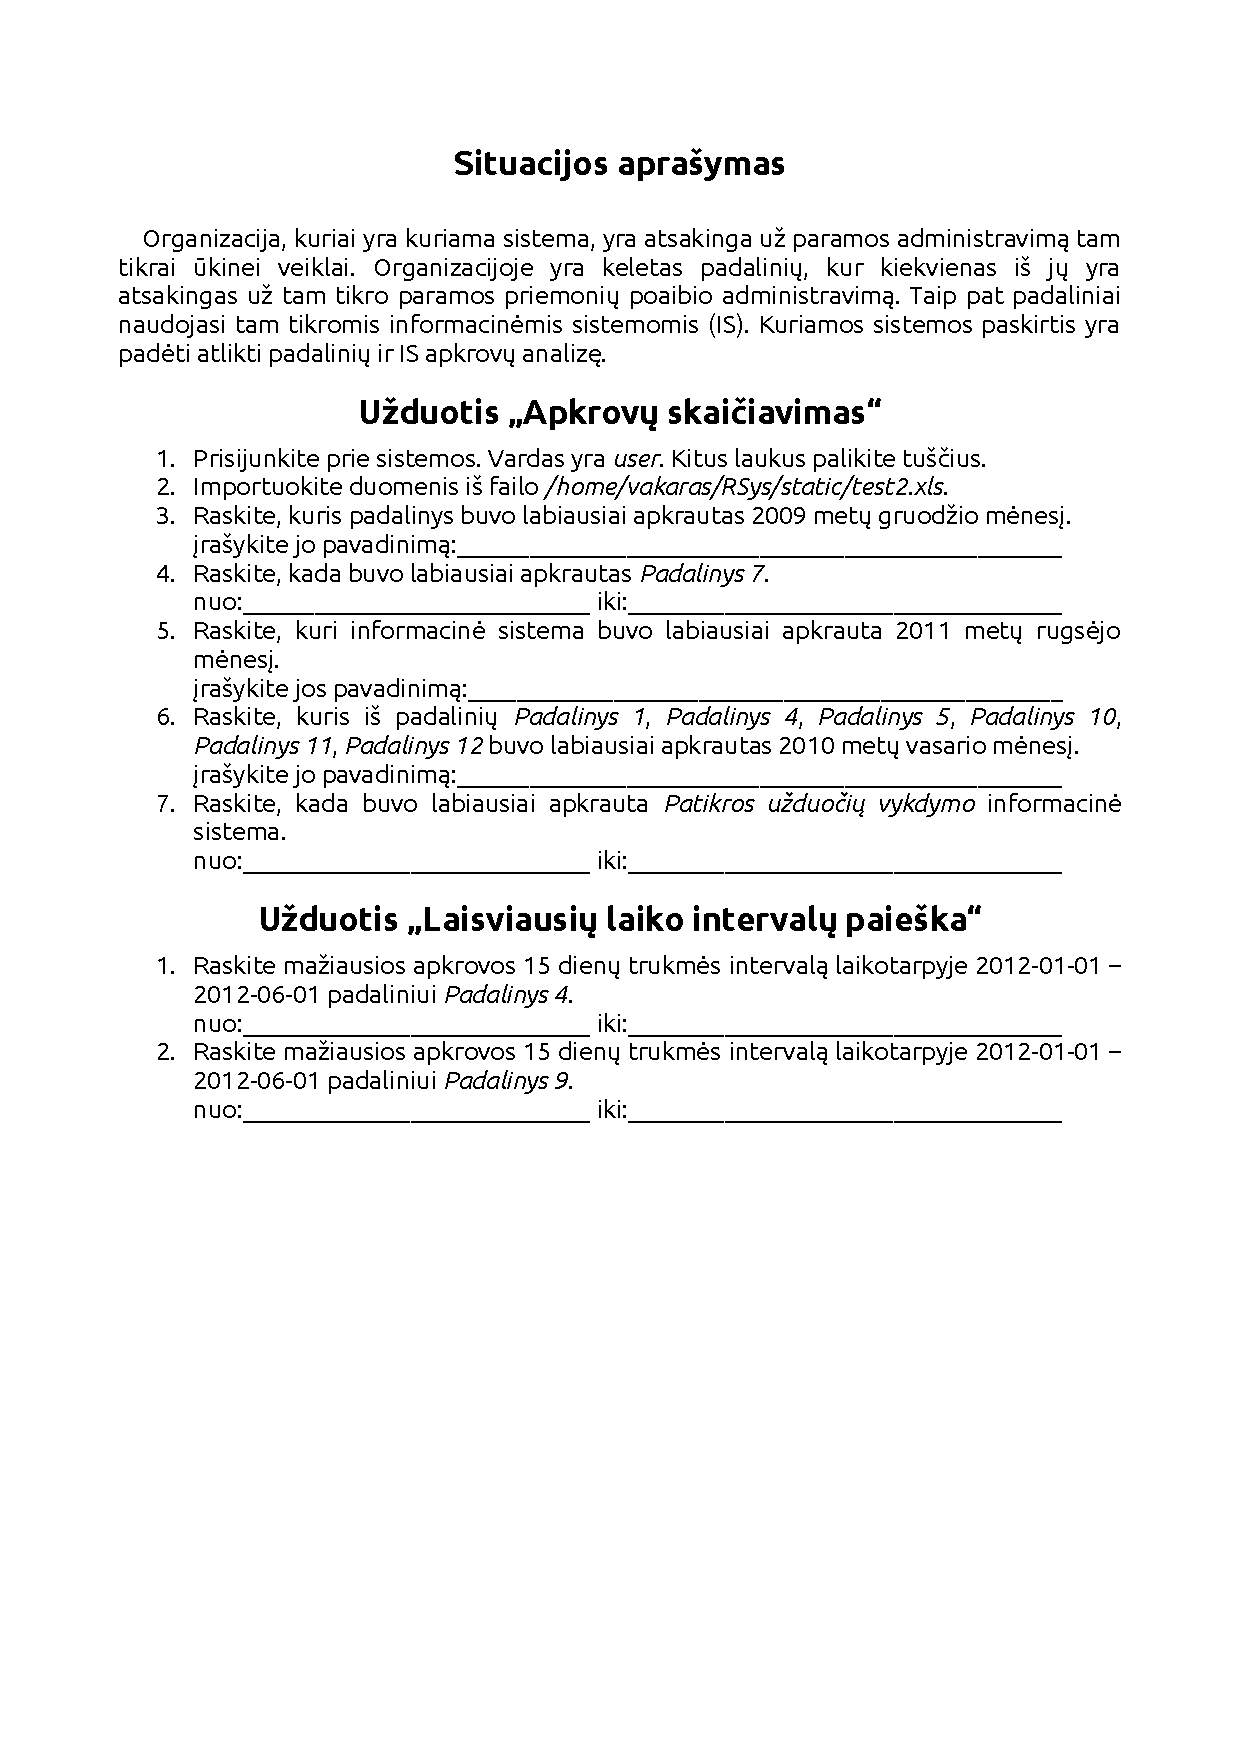
\includegraphics[scale=1.00]{./4/pdfs/task.pdf}

\newpage
\xsection{Priedas nr. 5: Dalyvių rezultatų lentelės}

\xsmallsec{Testuotojo A pirmos užduoties vykdymo rezultatai}

\xtable
{
  w [ 1 | 1 | 1 | 5 ]
  a [ p | p | p | p ]
  h [ Dalis | Laikas | Baigimas | Nesėkmės priežastis ]
  e [ 1 | 0:15 | Sėkmingas | ]
  e [ 2 | 0:54 | Sėkmingas | ]
  e [ 3 | 3:43 | Neteisingas atsakymas |
    Testuotojas nerado galimybės palyginti skirtingų padalinių apkrovas
    viename grafike ir bandė atspėti rezultatą lygindamas skirtingus
    grafikus.
    ]
  e [ 4 | 4:43 | Sėkmingas | ]
  e [ 5 | 3:41 | Neteisingas atsakymas |
    Sąlygoje buvo prašoma surasti labiausiai apkrautą IS, o rado
    labiausiai apkrautą padalinį.
    ]
  e [ 6 | 0:45 | Sėkmingas | ]
  e [ 7 | 2:46 | Sėkmingas | ]
}

\xsmallsec{Testuotojo B pirmos užduoties vykdymo rezultatai}

\xtable
{
  w [ 1 | 1 | 1 | 5 ]
  a [ p | p | p | p ]
  h [ Dalis | Laikas | Baigimas | Nesėkmės priežastis ]
  e [ 1 | 0:00 | Sėkmingas | ]
  e [ 2 | 0:31 | Sėkmingas | ]
  e [ 3 | 2:20 | Sėkmingas | ]
  e [ 4 | 5:23 | Neteisingas atsakymas |
    Testuotojas spėjo remdamasis grafiku. (Nežiūrėjo į lentelę.)
    ]
  e [ 5 | 3:05 | Sėkmingas | ]
  e [ 6 | 0:52 | Sėkmingas | ]
  e [ 7 | 2:52 | Sėkmingas | ]
}

\xsmallsec{Testuotojo C pirmos užduoties vykdymo rezultatai}

\xtable
{
  w [ 1 | 1 | 1 | 5 ]
  a [ p | p | p | p ]
  h [ Dalis | Laikas | Baigimas | Nesėkmės priežastis ]
  e [ 1 | 0:00 | Sėkmingas | ]
  e [ 2 | 0:59 | Sėkmingas | ]
  e [ 3 | 8:01 | Sėkmingas | ]
  e [ 4 | 2:05 | Sėkmingas | ]
  e [ 5 | 1:55 | Neteisingas atsakymas |
    Sąlygoje buvo prašoma surasti labiausiai apkrautą IS, o rado
    labiausiai apkrautą padalinį.
    ]
  e [ 6 | 1:58 | Sėkmingas | ]
  e [ 7 | 3:48 | Neteisingas atsakymas |
    Užrašė gretimo mėnesio datą.
    ]
}

\xsmallsec{Testuotojo D pirmos užduoties vykdymo rezultatai}

\xtable
{
  w [ 1 | 1 | 1 | 5 ]
  a [ p | p | p | p ]
  h [ Dalis | Laikas | Baigimas | Nesėkmės priežastis ]
  e [ 1 | 0:29 | Sėkmingas | ]
  e [ 2 | 1:09 | Sėkmingas | ]
  e [ 3 | 3:22 | Neteisingas atsakymas |
    Testuotojas nerado galimybės palyginti skirtingų padalinių apkrovas
    viename grafike ir bandė atspėti rezultatą lygindamas skirtingus
    grafikus.
    ]
  e [ 4 | 8:48 | Neteisingas atsakymas |
    Nesuprato užduoties. Nepastebėjo, kad yra duomenų ir už grafike
    rodomos srities.
    ]
  e [ 5 | 2:02 | Sėkmingas | ]
  e [ 6 | 2:28 | Sėkmingas | ]
  e [ 7 | 8:50 | Neteisingas atsakymas |
    Nesuprato užduoties. Nepastebėjo, kad yra duomenų ir už grafike
    rodomos srities.
    ]
}

\xsmallsec{Testuotojo E pirmos užduoties vykdymo rezultatai}

\xtable
{
  w [ 1 | 1 | 1 | 5 ]
  a [ p | p | p | p ]
  h [ Dalis | Laikas | Baigimas | Nesėkmės priežastis ]
  e [ 1 | 0:00 | Sėkmingas | ]
  e [ 2 | 0:43 | Sėkmingas | ]
  e [ 3 | 5:23 | Sėkmingas | ]
  e [ 4 | 1:18 | Sėkmingas | ]
  e [ 5 | 2:53 | Sėkmingas | ]
  e [ 6 | 2:12 | Sėkmingas | ]
  e [ 7 | 3:09 | Sėkmingas | ]
}

\xsmallsec{Naudotojų pirmos užduoties dalių vykdymo laikai}

\xtable
{
  w [ 1 | 1 | 1 | 1 | 1 | 1 ]
  a [ p | p | p | p | p | p ]
  h [ Dalis | A | B | C | D | E ]
  %
  e [ 1 | 0:15 | 0:00 | 0:00 | 0:29 | 0:00 ]
  e [ 2 | 0:54 | 0:31 | 0:59 | 1:09 | 0:43 ]
  e [ 3 | 3:43 | 2:20 | 8:01 | 3:22 | 5:23 ]
  e [ 4 | 4:43 | 5:23 | 2:05 | 8:48 | 1:18 ]
  e [ 5 | 3:41 | 3:05 | 1:55 | 2:02 | 2:53 ]
  e [ 6 | 0:45 | 0:52 | 1:58 | 2:28 | 2:12 ]
  e [ 7 | 2:46 | 2:52 | 3:48 | 8:50 | 3:09 ]
}
